\documentclass[10pt,landscape,a4paper]{article}
\usepackage{multicol}
\usepackage[landscape]{geometry}
\usepackage{hyperref}
\usepackage[utf8]{inputenc}
\usepackage{minted}
\usepackage{graphicx}
\usepackage{graphicx}


\geometry{top=0.5cm,left=0.5cm,right=0.5cm,bottom=0.5cm}

% Turn off header and footer
\pagestyle{empty}
 
% Redefine section commands to use less space
\makeatletter
\renewcommand{\section}{\@startsection{section}{1}{0mm}%
                                {-1ex plus -.5ex minus -.2ex}%
                                {0.5ex plus .2ex}%x
                                {\normalfont\large\bfseries}}
\renewcommand{\subsection}{\@startsection{subsection}{2}{0mm}%
                                {-1explus -.5ex minus -.2ex}%
                                {0.5ex plus .2ex}%
                                {\normalfont\small\bfseries}}
\renewcommand{\subsubsection}{\@startsection{subsubsection}{3}{0mm}%
                                {-1ex plus -.5ex minus -.2ex}%
                                {1ex plus .2ex}%
                                {\normalfont\footnotesize\bfseries}}
\makeatother

% Don't print section numbers
\setcounter{secnumdepth}{0}

\setlength{\parindent}{0pt}
\setlength{\parskip}{0pt plus 0.5ex}

\newcommand{\java}[1]{\mintinline{java}{#1}}


% -----------------------------------------------------------------------

\begin{document}

\footnotesize
\begin{multicols*}{3}


% multicol parameters
% These lengths are set only within the two main columns
%\setlength{\columnseprule}{0.25pt}
\setlength{\premulticols}{1pt}
\setlength{\postmulticols}{1pt}
\setlength{\multicolsep}{1pt}
\setlength{\columnsep}{2pt}


\section{Varia}

\begin{description}
\item[Initialisierung] Lokale Variablen explizit; Instanz-Variablen auch
  implizit mit default (false/0/null/...)
\item[Sichtbarkeit] \java{public}: alle Klassen, \java{protected}: package und
  sub-Klassen, \textvisiblespace: package, \java{private}: nur eigene Klasse
\item[Javadoc] \java{/** ... */}, \java{@author}, \java{@version}, \java{@param name}, \java{@return}, \java{@throws type}, \java{@deprecated}, \java{{@code}}, \java{@see}
\item[Package import conflicts] Eigene class $>$ \java{import p2.A} $>$ \java{package p1; class A} $>$ \java{import p2.*}
\item[Lambdas] \java{(Type o1, Type2 o2) -> {return o1.x() - o2.x()}} \\
  $\Rightarrow$ \java{(o1, o2) -> o1.x() - o2.x()}
\item[String API] \java{.charAt}, \java{.startsWith}, \java{.replace}, \java{.length()} \\ \java{new StringBuilder(s).reverse().toString()}
\item[iterieren] \java{for (int val : arr) { ... }}, \\ \java{Iterator<t> it = coll.iterator(); it.hasNext();} \\ \java{it.next(); it.remove()}
\end{description}

\section{equals / hashcode}

\begin{minted}{java}
@Override
public boolean equals(Object obj) {
  if (obj == null || getClass() != obj.getClass()) {
    return false; }
  // if (!super.equals(obj))  { return false; }
  Student other = (Student)obj;
  return getRegNumber() == other.getRegNumber() }
public int hashCode() {  /* @Override */
  return f1.hashCode() + 31 * f2.hashCode() }
\end{minted}

\section{compareTo}

\begin{minted}{java}
class Student implements Comparable<Student> {
  @Override
  public int compareTo(Student other) {
    return regNumber - other.regNumber;
    // oder z.B. compareTo auf Nachname-String,
    // falls 0 auch auf Vorname
  }}
\end{minted}

\section{clone}

\begin{minted}{java}
class Person implements Cloneable {
  @Override
  public Person clone() {
    return new Person(firstName, lastName); }}
  // CloneNotSupportedException
\end{minted}

\section{JUnit}

\begin{minted}{java}
public class StackTest {
  @Before // @After, @BeforeClass, @AfterClass
  public void setUp() {...}
  @Test(timeout = 10) // ms
  // @Test(expected = MyException.class)
  public void testFoo() {
    assertEquals("kaputt", expected, actual);
    assertFalse("kaputt", v);
    fail(); }}
\end{minted}

Methoden wie PyUnit, aber \verb|Same| statt \verb|Is| und \verb|Null| statt \verb|None|.

\section{Exception}

\begin{minted}{java}
class MyException extends Exception {
  private static final long serialVersionUID = ...L;
  MyException(String message) {
    super(message);
  }
}
public String clip(String s) throws MyException {
  throw new MyException("bla");
}
try {
  s = clip(s);
} catch (MyException | OtherException) {
  e.getMessage();
  e.printStackTrace();
}
\end{minted}

\section{Collections}

\begin{minted}{java}
Map<KType, VType> map = new HashMap<>();
// TreeMap: sortiert, etwas langsamer
map.put(100, obj); map.get(100);
map.containsKey(100);
map.values(); map.entrySet().toArray();
for (Map.entry<K, V> entry: map.entrySet()) {
  e.getKey(); e.getValue();
}

List<T> list = new ArrayList<>();  // LinkedList
list.add(obj); list.get(0);
list.addAll(list2); list.remove(0);
list.size();
Collections.sort(list[, Comparator]);

Set<T> set = new HashSet<>();  // TreeSet: wie TreeMap
set.add(obj); set.contains(obj);
set.size();
\end{minted}

\section{Generics}

\begin{minted}{java}
class Pair<T, U> {
  private final T first; // + second
  public T getFirst() { ... } // + second
}
class Foo<T extends Type1 & Type2>
<T extends Comparable<T>> boolean isAsc(T[] arr) { ... }
\end{minted}

\section{Dynamic dispatch}

\begin{minted}{java}
class Base { public void copyTo(Base other) { (1) } }
class Sub extends Base {
  public void copyTo(Base other) { (2) }
  public void copyTo(Sub other) { (3) }
}
Base b = new Sub(); Sub s = new Sub();
b.copyTo(b); // 2 (dynamic dispatch)
b.copyTo(s); // 2 (Compiler kennt overload nicht)
((Base)s).copyTo(s) // 2
s.copyTo(b); s.copyTo(s); // 2, 3
\end{minted}

Bei private-Methoden: Kein dynamic dispatch!

\section{Comparator-Bausteine}

\begin{minted}{java}
people.sort(Comparator.comparing(P::meth1).
            thenComparing(P::meth2).reversed())
\end{minted}

\section{Stream API}
\begin{minted}{java}
building.stream()
  .filter(p -> p instanceof House)
  .map(p -> (House)p.address())
  .sorted((a, b) -> a.foo() - b.foo()).distinct()
  .skip(5).limit(10)
  .forEach(System.out::println)
// OptionalDouble: .isPresent() .getAsDouble() .ifPresent(x)
people.stream().mapToInt(p -> p.getAge()).average()
\end{minted}


\section{I/O Streams}
\subsection{Byte Streams}
\begin{minted}{java}
try (FileInputStream fis = new FIS("input.txt")) {
  int value = fis.read();
  while (value >= 0) {
    byte b = (byte)value;
    // Use b
    value = fis.read(); }
} catch (IOException e) {
  // also: FileNotFoundException
}

try (FileOutputStream fos = new FOS("output.txt")) {
  byte b = ...;
  fos.write(b);
} // implizit .flush(), .close()
\end{minted}
\subsection{Andere}

\begin{description}
  \item[character] Wie oben, \java{FileReader} und \java{FileWriter}, mit \java{char} als Typ, und \java{reader.getEncoding()}
  \item[bridge] \java{Reader r = new InputStreamReader(byteSt, "UTF-8")}
  \item[buffered in] \java{BufferedReader r = new BR(filereader);},
    \java{String s = r.readLine();}, \java{null} bei EOF.
  \item[buffered out] \java{BufferedOutputStream s = new BOS(fos, 4096);}
  \item[appending] \java{true} als zweites Argument mitgeben
\end{description}

\section{Serializing}

\begin{minted}{java}
class Person implements Serializable {
  private String foo;
  private transient int age;  // nicht serialisiert
  private (...) serialVersionUID = 1L;
} // else: NotSerializableException

Person person = new Person();
OutputStream fos = new FileOutputStream("person.bin");
try (ObjectOutputStream s = new OOS(fos)) {
  stream.writeObject(person);
}

InputStream fis = new FileInputStream("person.bin");
try (ObjectInputStream s = new ObjectInputStream(fis)) {
  Person p = (Person)stream.readObject();
} // falsche Version: ClassNotFoundException
\end{minted}

\section{Interfaces / Abstract classes}

\subsection{Interface}
\begin{minted}{java}
interface If1 {
  int IMPLIZIT_CONST_FINAL = 1;
  void foo();  // implizit public abstract
  default void defaultMeth() { ... }}
class Foo implements If1, If2 extends Superclass
\end{minted}

\subsection{FunctionalInterface}
\begin{minted}{java}
@FunctionalInterface
interface Comparator<T> { int compare(T a, T b); }

java.util.function.Predicate<T> boolean test(T t)
Supplier<T> T get()
Consumer<T> void accept(T t)
Function<T, R> R apply(T t)
\end{minted}

\subsection{Abstract class}

\begin{minted}{java}
abstract class Vehicle {
  abstract void report();
  void print() { ... }
}
\end{minted}

\section{Rekursion}

recursion \emph{n.} See $\rightarrow$ recursion.

\subsection{Fibonacci}

\begin{minted}{java}
static double fib(double n) {
  if (n == 0) { return 0; }
  else if (n == 1) { return 1; }
  else { return fib(i - 1) + fib(i - 2); }
}
\end{minted}

\subsection{Hanoi}
\begin{minted}{java}
public void solve(int n, String start, String tmp,
  if (n == 1) {   String end) {
    sysout(start + " -> " + end);
  } else {
    solve(n - 1, start, end, tmp);
    sysout(start + " -> " + end);
    solve(n - 1, tmp, start, end);
  }} foo.solve(count, "A", "B", "C");
\end{minted}

\subsection{Labyrinth}
\begin{minted}{java}
static boolean[][] visited = ...;
static boolean findPath(int x, int y, String path) {
  path += "-> [" + x + ", " + y + "] ";
  if (!isAccessible(x, y) || visited[x][y]) {
    return false;
  } else if (x == targetX && y == targetY) {
    System.out.println(path);
    return true;
  } else {
    visited[x][y] = true;
    boolean found = findPath(x - 1, y, path) ||
      findPath(x + 1, y, path) ||
      findPath(x, y - 1, path) ||
      findPath(x, y + 1, path);
    visited[x][y] = false; }}
\end{minted}

\section{Operator precedence}
\verb|+|, \verb|-| (unary), \verb|++|, \verb|--| \hspace{1em}
\verb|*|, \verb|/|, \verb|%| \hspace{1em}
\verb|+|, \verb|-| \\
\verb|<|, \verb|<=|, \verb|>|, \verb|>=| \hspace{1em}
\verb|==|, \verb|!=| \hspace{1em}
\verb|&&| \hspace{1em}
\verb&||& \\
Achtung: Short-circuit bei \verb|a && b| und \verb&a || b&!

\section{Enums}
\begin{minted}{java}
public enum Weekday {
  MONDAY, TUESDAY, WEDNESDAY, ...;
  public boolean isMonday() { return this == Monday; }}
Weekday today = Weekday.MONDAY;
\end{minted}

\section{Scanner}
\begin{minted}{java}
try (Scanner scanner = new Scanner(System.in)) {
  while (scanner.hasNextLine()) {
    scanner.nextInt(); .nextDouble(); .nextFloat();
    scanner.next(); }} // String
\end{minted}

\section{Vergleiche}
\begin{description}
  \item[primitiv] \java{v1 == v2;}
  \item[strings] \java{s1.equals(v2);}
  \item[arrays] \java{Arrays.equals(a, b); Arrays.deepEquals(a, b);}
\end{description}

\section{Zirkulare Referenzen verhindern}
\begin{minted}{java}
public void add(Item item) {
  if (contains(item, this)) { throw ...; }
  else { this.bundle.add(item); } }
private boolean contains(Item needle, Item haystack) {
  if (needle.equals(haystack)) {
    return true;
  } else if (haystack instanceof BundleItem) {
    for (Item child : ((BundleItem)haystack).bundle) {
      if (contains(needle, child)) {
        return true; }}}
  return false; }
\end{minted}

\section{Casts}
\begin{minted}{java}
Vehicle v = new Car(); // impliziter upcast (Liskov)
Object o = new Car();  // expliziter downcast
Car c = (Car)o;
Vehicle v = new Vehicle();  // !(v instanceof Car)
Car c = (Car)v;             // -> exception 
\end{minted}

\begin{multicols*}{2}
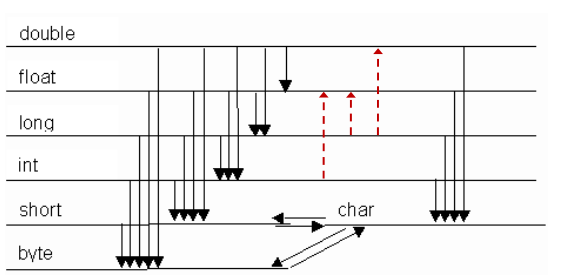
\includegraphics[width=\columnwidth]{casts.png} \\
schwarz: explizit, rot: implizit (ggf. Genauigkeitsverlust), \\ andere implizit
\section{Collections}
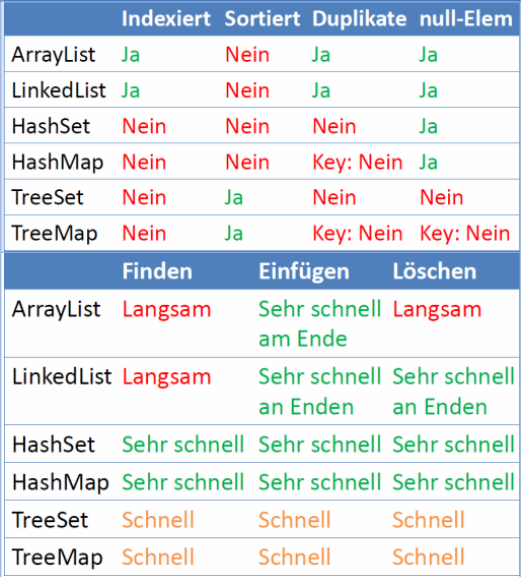
\includegraphics[width=\columnwidth]{collections.png}
\end{multicols*}

\section{Linked Person}

\begin{minted}{java}
boolean isLinked(Person from, Person to) {
  return isLinked(from, to, new HashSet<>()); }
boolean isLinked(Person from, Person to,
                 Set<Person> visited) {
 if (from == to) { return true; }
 if (visited.contains(from)) { return false; }
 visited.add(from);
 for (Person other : from.getKnownPeople()) {
   if (isLinked(other, to, visited)) { return true; }
 } return false; }
\end{minted}

\section{Knights tour}

\begin{minted}{java}
private final int[][] board = new int[NOF_ROWS][NOF_COLS];
private final int[][] moves = {{-1,-2},{-1,+2},{+1,-2},
  {+1,+2},{-2,-1},{-2,+1},{+2,-1},{+2,+1}};
private boolean findTour(int x, int y, int step) {
  if (insideBoard(x, y)) {
    if (step == NOF_ROWS * NOF_COLS) {
      return board[x][y] == 1; // closed tour
    } else if (board[x][y] == FREE) {
      board[x][y] = step + 1;
      int[][] next = nextPositions(x, y);
      for (int k = 0; k < next.length; k++) {
        if (findTour(next[k][0], next[k][1], step + 1)) {
          return true;
        }
      }
      board[x][y] = FREE;
    }
  }
  return false;
}
private int[][] nextPositions(int x, int y) {
 int[][] next = new int[moves.length][];
 for (int k = 0; k < moves.length; k++) {
   next[k] = new int[] { x + moves[k][0],
                         y + moves[k][1] };
 } return next;
}
private boolean insideBoard(int x, int y) {
 return x >= 0 && x < NOF_ROWS && y >= 0 && y < NOF_COLS;
}
\end{minted}

\section{Datentypen}
\begin{tabular}{llll}
  char & 16bit & UTF-16 & \java{'x'} \\
  byte & 8bit & $-127\ldots128$ & \\
  short & 16bit & $-32768\ldots32757$ & \\
  int & 32bit & $-2^{31}\ldots2^{31}-1$ & \java{23} \\
  long & 64bit & $-2^{63}\ldots2^{63}-1$ & \java{23l} \\
  float & 32bit & & \java{0.f}, \java{2e4f} \\
  double & 64bit & & \java{0.1}, \java{2e4}
\end{tabular}

\begin{itemize}
\item 1/0: \java{ArithmeticException}
\item 0/0.0: \java{NaN}
\item 1/0.0: \java{Double.POSITIVE_INFINITY}
\item -1/0.0: \java{Double.NEGATIVE_INFINITY}
\item Float comparison: \java{Math.abs(a - b) < 1e-8}
\end{itemize}

\end{multicols*}
\end{document}